%% General definitions
\documentclass{article} %% Determines the general format.
\usepackage{a4wide} %% paper size: A4.
\usepackage[utf8]{inputenc} %% This file is written in UTF-8.
%% Some editors on Windows cannot save files in UTF-8.
%% If there is a problem with special characters not showing up
%% correctly, try switching "utf8" to "latin1" (ISO 8859-1).
\usepackage[T1]{fontenc} %% Format of the resulting PDF file.
\usepackage{fancyhdr} %% Package to create a header on each page.
\usepackage{lastpage} %% Used for "Page X of Y" in the header.
                      %% For this to work, you have to call pdflatex twice.
\usepackage{enumerate} %% Used to change the style of enumerations (see below).

\usepackage{amssymb} %% Definitions for math symbols.
\usepackage{amsmath} %% Definitions for math symbols.

\usepackage{tikz}  %% Pagacke to create graphics (graphs, automata, etc.)
\usetikzlibrary{automata} %% Tikz library to draw automata
\usetikzlibrary{arrows}   %% Tikz library for nicer arrow heads
\usetikzlibrary{positioning}    %% Tikz library for more positioning options

\usepackage{hyperref} %% hyperlinks

\usepackage{chessfss} % contained in debian package texlive-games

\tikzset{WhiteSquare/.style = {shape=rectangle, minimum width=28, minimum
    height=28, anchor=south west}}
\tikzset{BlackSquare/.style = {shape=rectangle, fill=lightgray, minimum
    width=28, minimum height=28, anchor=south west}}

%% Left side of header
\lhead{\course\\\semester\\Exercise \homeworkNumber}
%% Right side of header
\rhead{\authorname\\Page \thepage\ of \pageref{LastPage}}
%% Height of header
\usepackage[headheight=36pt]{geometry}
%% Page style that uses the header
\pagestyle{fancy}

\newcommand{\authorname}{Benjamin Regez\\Luis Tritschler}
\newcommand{\semester}{Spring Semester 2026}
\newcommand{\course}{Foundations of Artificial Intelligence}
\newcommand{\homeworkNumber}{6}

\renewcommand{\thesection}{Exercise \homeworkNumber.\arabic{section}}


\begin{document}

\section{}
\begin{enumerate}[(a)]
    \item \textit{COP of finding a maximum Hamiltonian
    path in a fully connected graph}\\[0.5em]
    $\mathcal{O} = \langle C, S, \text{opt}, \text{v} \rangle$ with
    \begin{itemize}
        \item $C = \{
            \langle V, E \rangle \ | \
            V \in \langle v_1, v_2, ..., v_n, v_{n+1} \rangle, \
            n \in \mathbb{N}, \
            v_{n+1} = v_1, \
            E = \{ \langle v_i, v_{i+1} \rangle \ | \ i \in \{ 1, ..., n \} \}
        \}$
        \item $S = \{
            \langle V, E \rangle \in C \ | \
            w(v_k, v_{k+1}) \in \mathbb{R^+}
            \}$
        \item opt = max
        \item $v(S) = \sum_{k=1}^{n} w(v_k, v_{k+1}) $
    \end{itemize}
    \item We state that for a given problem instance, there might exist several solutions with maximum edge weight sum.\\
    That means, the problem consists of both finding a solution (search) as well as
    finding the maximum (optimization). Thus, \textit{maximum Hamilton path}
    is a combined search and optimization problem according to our formulation in (a).
    \item We define the neighborhood function \texttt{neigh} as follows:\\[0.5em]
    \texttt{neigh}$(
        \{
            \langle V, E \rangle \in C \ | \
            V = \langle v_1, v_2, ..., v_l, ..., v_m, ... v_n, v_{n+1} \rangle , \
            l < m, \
            l, m \in \{ 1, ..., n \}
        \}
        ) \\[0.4em]
    = \{
        \langle V, E \rangle \ | \
        V = \langle v_1, v_2, ..., v_m, ..., v_l, ... v_n, v_{n+1} \rangle
    \}$
\end{enumerate}

\section{}
% 
Remark: Numbers in tiles indicate the heuristic of the neighbor (if the queen in this file is moved to this tile).
\begin{enumerate}[(a)]
    \item Hill Climbing with heuristic and neighborhood from slide C1 p. 23.\\
    Initial candidate (current heuristic value: 3):
\begin{center}
  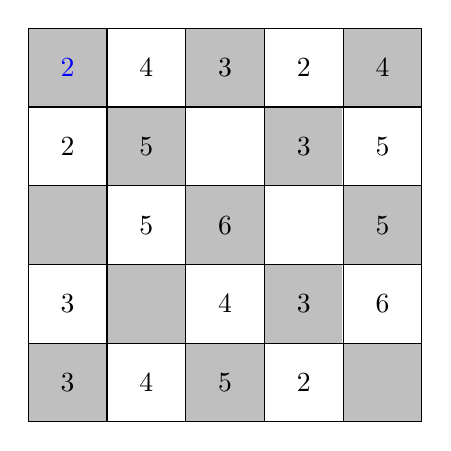
\begin{tikzpicture}
    \draw[step=1,black,thin] (0,0) grid (5,5);

    % First file
    \node[BlackSquare] at (0,0) {3}; 
    \node[WhiteSquare] at (0,1) {3};
    \node[BlackSquare] at (0,2) {\BlackQueenOnWhite};
    \node[WhiteSquare] at (0,3) {2};
    \node[BlackSquare] at (0,4) {\color{blue}2\color{black}};
    
    % Second file   
    \node[WhiteSquare] at (1,0) {4};
    \node[BlackSquare] at (1,1) {\BlackQueenOnWhite};
    \node[WhiteSquare] at (1,2) {5};
    \node[BlackSquare] at (1,3) {5};
    \node[WhiteSquare] at (1,4) {4};

    % Third file 
    \node[BlackSquare] at (2,0) {5};
    \node[WhiteSquare] at (2,1) {4};
    \node[BlackSquare] at (2,2) {6};
    \node[WhiteSquare] at (2,3) {\BlackQueenOnWhite};
    \node[BlackSquare] at (2,4) {3};

    % Fourth file
    \node[WhiteSquare] at (3,0) {2};
    \node[BlackSquare] at (3,1) {3};
    \node[WhiteSquare] at (3,2) {\BlackQueenOnWhite};
    \node[BlackSquare] at (3,3) {3};
    \node[WhiteSquare] at (3,4) {2};

    % Fifth file
    \node[BlackSquare] at (4,0) {\BlackQueenOnWhite};
    \node[WhiteSquare] at (4,1) {6};
    \node[BlackSquare] at (4,2) {5};
    \node[WhiteSquare] at (4,3) {5};
    \node[BlackSquare] at (4,4) {4};

    \end{tikzpicture}
\end{center}
First iteration (current heuristic value: 2):
\begin{center}
  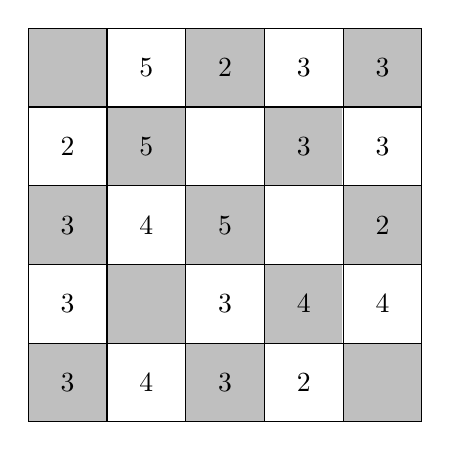
\begin{tikzpicture}
    \draw[step=1,black,thin] (0,0) grid (5,5);

    % First file
    \node[BlackSquare] at (0,0) {3}; 
    \node[WhiteSquare] at (0,1) {3};
    \node[BlackSquare] at (0,2) {3};
    \node[WhiteSquare] at (0,3) {2};
    \node[BlackSquare] at (0,4) {\BlackQueenOnWhite};
    
    % Second file   
    \node[WhiteSquare] at (1,0) {4};
    \node[BlackSquare] at (1,1) {\BlackQueenOnWhite};
    \node[WhiteSquare] at (1,2) {4};
    \node[BlackSquare] at (1,3) {5};
    \node[WhiteSquare] at (1,4) {5};

    % Third file 
    \node[BlackSquare] at (2,0) {3};
    \node[WhiteSquare] at (2,1) {3};
    \node[BlackSquare] at (2,2) {5};
    \node[WhiteSquare] at (2,3) {\BlackQueenOnWhite};
    \node[BlackSquare] at (2,4) {2};

    % Fourth file
    \node[WhiteSquare] at (3,0) {2};
    \node[BlackSquare] at (3,1) {4};
    \node[WhiteSquare] at (3,2) {\BlackQueenOnWhite};
    \node[BlackSquare] at (3,3) {3};
    \node[WhiteSquare] at (3,4) {3};

    % Fifth file
    \node[BlackSquare] at (4,0) {\BlackQueenOnWhite};
    \node[WhiteSquare] at (4,1) {4};
    \node[BlackSquare] at (4,2) {2};
    \node[WhiteSquare] at (4,3) {3};
    \node[BlackSquare] at (4,4) {3};

    \end{tikzpicture}
\end{center}
The algorithm already stops after the first iteration, because the heuristic value
of the current candidate is 2 and there is no tile with a better heuristic value.

\newpage
    \item Hill climbing variant where the next candidate that is considered is selected
by first picking a file at random and then moving the (unique) queen in that file to a square
in that file with the best heuristic value (the variant is introduced on slide 9 of Chapter C2
in the print version of the lecture slides). Assume that the random choices are resolved in
such a way that the file selection picks the third file first, and in each subsequent step the file
that is to the left of the file that was selected last (if the leftmost file was selected last, the
rightmost file is selected).\\[0.5em]
\color{red}TODO \color{black}
\end{enumerate}

\newpage
\section{}


\section{}


\section{}


\section*{Statement on scientific integrity}
The following prompts were entered into Copilot:
\begin{itemize}
    \item (Ex 6.1(a)) "wie gebe ich mathematisch korrekt in einem undirected graph das gewicht w eines edges e an?"
\end{itemize}
% Google Translate was used to assist in translating individual words from
% German to English when writing down the exercise solutions.\\
Apart from that, we solved the entire exercise sheet on our own.

\end{document}
